\documentclass[a4paper,12pt]{report}
\usepackage{multicol}
\usepackage[toc,page]{appendix}
\usepackage{amsmath}
\usepackage{float}
\usepackage{graphicx}
\usepackage{subfig}
\usepackage{amssymb}
\usepackage{geometry}
\usepackage{setspace}
\usepackage{soul}
\usepackage{tcolorbox}
\usepackage{multirow}% http://ctan.org/pkg/multirow
 \geometry{
 a4paper,
 total={170mm,257mm},
 left=20mm,
 top=20mm,
 }
\usepackage{tikz}
\usepackage{pgfplots}
\usetikzlibrary{shapes, arrows.meta, decorations.pathreplacing, positioning, petri, fit, calc}
\tikzstyle{startstop} = [rectangle, rounded corners, minimum width=2cm, minimum height=0.5cm,text centered, text width=3cm, draw=black, fill=gray!30]
\tikzstyle{process} = [rectangle, minimum width=2cm, minimum height=0.5cm, text centered, text width=3cm, draw=black, fill=blue!30]
\tikzstyle{detail} = [rectangle, minimum width=7cm, minimum height=0.5cm, text justified, text width=6.5cm, fill=white!30]
\tikzstyle{smalldetail} = [rectangle, minimum width=3.5cm, minimum height=0.5cm, text justified, text width=3cm, draw=white, fill=white!30]
\tikzstyle{decision} = [rectangle, minimum width=1.5cm, minimum height=1cm, text centered, draw=black, fill=green!30]
\tikzstyle{neuron} = [circle, minimum size=1cm ,text centered, draw=red, fill=gray!30]
\usepackage[utf8]{inputenc}

% Default fixed font does not support bold face
\DeclareFixedFont{\ttb}{T1}{txtt}{bx}{n}{10} % for bold
\DeclareFixedFont{\ttm}{T1}{txtt}{m}{n}{10}  % for normal

% Custom colors
\usepackage{color}
\definecolor{deepblue}{rgb}{0,0,0.5}
\definecolor{deepred}{rgb}{0.6,0,0}
\definecolor{deepgreen}{rgb}{0,0.5,0}

\usepackage{listings}

% Python style for highlighting
\newcommand\pythonstyle{\lstset{
language=Python,
basicstyle=\ttm,
otherkeywords={self},             % Add keywords here
keywordstyle=\ttb\color{deepblue},
emph={MyClass,__init__},          % Custom highlighting
emphstyle=\ttb\color{deepred},    % Custom highlighting style
stringstyle=\color{deepgreen},
%frame=tb,                         % Any extra options here
showstringspaces=false            % 
}}
\newcommand{\code}[1]{\texttt{#1} }

% Python environment
\lstnewenvironment{python}[1][]
{
\pythonstyle
\lstset{#1}
}
{}

% Python for external files
\newcommand\pythonexternal[2][]{{
\pythonstyle
\lstinputlisting[#1]{#2}}}

% Python for inline
\newcommand\pythoninline[1]{{\pythonstyle\lstinline!#1!}}

\begin{document}
\tableofcontents

\title{Using Python to Access Web Data \\ University of Michigan \\ Charles Severance}
\maketitle
\part{Regular Expresion}
Regular expression is a concise and flexible means for matching string in a text.
\begin{table}[]
\centering
\label{}
\begin{tabular}{ll}
\^{}  & matches \textbf{begining} of a line   \\
 \$ &  matches \textbf{end} of a line  \\
 . &  matches any char \\
 \textbackslash s & matches \textbf{whitespace} \\
 \textbackslash S &  matches any \textbf{non-whitespace} char  \\
 * &   \textbf{repeats} a char zero or more times  \\
 *? &  \textbf{repeats} a char zero or more times (non greedy) \\
 $+$ & \textbf{repeats} a char one or more times \\ 
 $+$ ? & \textbf{repeats} a char one or more times (non greedy) \\ 
$[$aeiou$]$ & matches a single char \textbf{in} the listed \textbf{set}\\ 
$[$\^{}XYZ$]$ & matches a single char \textbf{not in} the list \textbf{set}\\ 
$[$a-z0-9$]$ & The set of character can include a \textbf{range} \\ 
( & indicates where string extraction is to start \\
) & indicates where string extraction is to end
\end{tabular}
\end{table}
\\

\section{\textit{re} library and functions}
\begin{table}[]
\centering
\label{}
\begin{tabular}{ll}
\code{Import re} &  import library \textit{re}   \\
 \code{re.search(patt, text)} &  see if a pattern matches is found in text (return TRUE/FALSE)  \\
 \code{re.findall(patt, text)} &  extract pattern if found in text \\
& (return a list with expression matching pattern)  \\
\end{tabular}
\end{table}
\subsection{Examples}

\begin{tcolorbox}
\begin{python}
if re.search('^From:', line)
	print line
\end{python}
\end{tcolorbox}

If the expression 'From:' is found at the beginning of a line (\^{}), return \textbf{\textcolor[rgb]{0,0.58,0}{TRUE}} and print the line.
\begin{tcolorbox}
\begin{python}
if re.search('^From:', line) 
	print line
% TRUE if 'From' is found at the begining of the line '^'
\end{python}
\end{tcolorbox}

\begin{tcolorbox}
\begin{python}
if re.search('^X.*:', line)
	print line
% TRUE if 'X' followed by any number of char (.) finishing with ':'
\end{python}
\end{tcolorbox}
\begin{tcolorbox}
\begin{python}
x = 'My 2 favorite numbers are 19 and 42'
y = re.findall('[0-9]+', x) % any number of digits
%Return ['2', '19', '42']
\end{python}
\end{tcolorbox}
\begin{tcolorbox}
\begin{python}
x = 'My 2 favorite numbers are 19 and 42'
y = re.findall('[AEIOU]+', x)  % 1 or more capital voyel
% Return []
\end{python}
\end{tcolorbox}

\subsection{Greedy Matching}
The repeats (* and +) tried to match the largest possible string (greedy).\\
\begin{tcolorbox}
\begin{python}
x = 'From: Using the : character'
y = re.findall('^F.+:', x)
print y
%Return ['From: using the :']
\end{python}
\end{tcolorbox}
For \textit{Non-greedy} match:\\
\begin{tcolorbox}
\begin{python}
x = 'From: Using the : character'
y = re.findall('^F.+?:', x)
print y
%Return ['From:']
\end{python}
\end{tcolorbox}

\subsection{Fine Tuning string extracting}
\begin{tcolorbox}
\begin{python}
x = 'From stephen.marquard@uct.ac.za Sat Jan 5 09:14:16 2008'
y = re.findall('\S+@\S+', x)
print y
%Return ['stephen.marquard@uct.ac.za']
\end{python}
\end{tcolorbox}

\begin{itemize}
\item Find a ligne starting with 'From', followed by a blank and match what's in '( )'
\begin{tcolorbox}
\begin{python}
x = 'From stephen.marquard@uct.ac.za Sat Jan 5 09:14:16 2008'
y = re.findall(^From (\S+@\S+)', x)
print y
%Return ['stephen.marquard@uct.ac.za']
\end{python}
\end{tcolorbox}
\end{itemize}

\begin{itemize}
\item Find domain name
\begin{tcolorbox}
\begin{python}
x = 'From stephen.marquard@uct.ac.za Sat Jan 5 09:14:16 2008'
y = re.findall('@([^ ]*', x)
print y
%Return ['uct.ac.za']
\end{python}
\end{tcolorbox}
'\^' in [ ] means NOT ('[\^ ] not white space character \\
' * ' match many no white space character
\end{itemize}

\begin{itemize}
\item If you want a special regular expression character to behave normally, use '\': \\
\begin{tcolorbox}
\begin{python}
\$[0-9.]+  % \$=real dollar
           % a digit or a '.' at least one or more
\end{python}
\end{tcolorbox}
\end{itemize}

\part{Networked Program}
\section{Sockets in Python}
Python built-in support for TCP sockets \\

\begin{figure}[H]
        \centering
        \resizebox {6in} {!} {
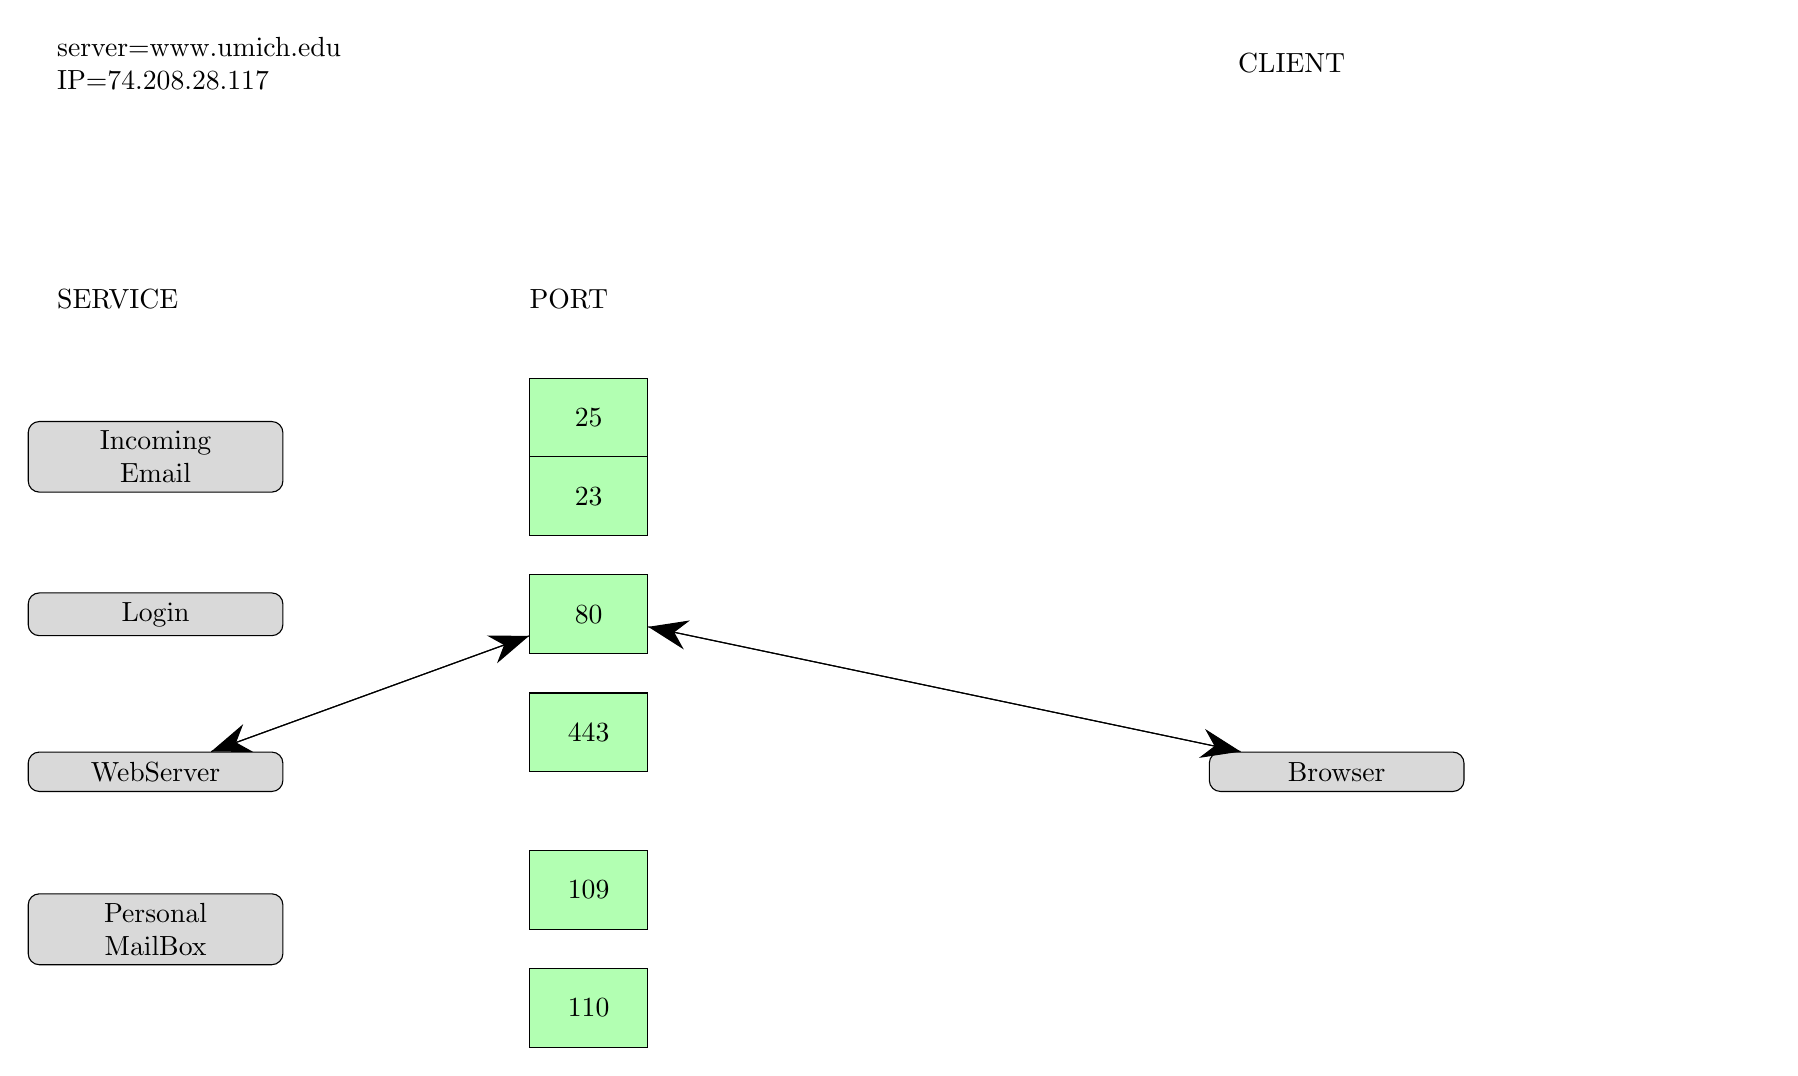
\begin{tikzpicture}[node distance=4cm]
\node (server) [detail] {server=www.umich.edu \\ IP=74.208.28.117};
\node (client) [detail,below of=server, xshift=15cm, yshift=4cm] {CLIENT};
\node (service) [detail,below of=server, xshift=0cm, yshift=1cm] {SERVICE};
\node (port) [detail, below of=server, xshift=6cm, yshift=1cm] {PORT};
\node (incomingEmail) [startstop, below of=service, xshift=-2cm, yshift=2cm] {Incoming \\ Email};
\node (login) [startstop, below of=incomingEmail, xshift=0cm, yshift=2cm] {Login};
\node (webserver) [startstop, below of=login, xshift=0cm, yshift=2cm] {WebServer};
\node (personalMailBox) [startstop, below of=webserver, xshift=0cm, yshift=2cm] {Personal \\ MailBox};
\node (p25) [decision, below of=port, xshift=-2.5cm, yshift=2.5cm] {25};
\node (p23) [decision, below of=p25, xshift=0cm, yshift=3cm] {23};
\node (p80) [decision, below of=p23, xshift=0cm, yshift=2.5cm] {80};
\node (p443) [decision, below of=p80, xshift=0cm, yshift=2.5cm] {443};
\node (p109) [decision, below of=p443, xshift=0cm, yshift=2cm] {109};
\node (p110) [decision, below of=p109, xshift=0cm, yshift=2.5cm] {110};
\node (browser) [startstop, below of=client, xshift=-2cm, yshift=-5cm] {Browser};

\draw[-{Stealth[length=5mm]}] (browser) -- (p80);
\draw[-{Stealth[length=5mm]}] (p80) -- (browser);
\draw[-{Stealth[length=5mm]}] (webserver) -- (p80);
\draw[-{Stealth[length=5mm]}] (p80) -- (webserver);

\end{tikzpicture}
}
\end{figure}

\begin{tcolorbox}
\begin{python}
import socket
mysock = socket.socket(socket.AF_INET, socket.SOCK_STREAM) %create a socket
mysock.connect( ('www.py4inf.com', 80) ) %connect socket to server
% HOST=www.py4inf.com and PORT=80
\end{python}
\end{tcolorbox}

\begin{tabular}{cccc}
URL & htpp:// &www.dr-chuck.com/ & page.htm \\
    & what protocol to use & host & document \\
\end{tabular}

\section{getting data from the server}
\subsection{Making a HTTP Request: the old way}
\begin{itemize}
\item Connect to the server (www.dr-chuck.com)
\item request a document: GET http://www.dr-chuck.com/page1.html
\end{itemize}

\begin{tcolorbox}
\begin{python}
import socket
mysock = socket.socket(socket.AF_INET, socket.SOCK_STREAM) %create a socket
mysock.connect( ('www.py4inf.com', 80) ) %connect socket to server
mysock.send('GET http://www.py4inf.com/code/romeo.txt HTTP/1.0\n\n'
while True:
	data = mysock.recv(512) %512 chars
	if( len(data) < 1 ): %end of file
		break
	print data
mysock.close()
\end{python}
\end{tcolorbox}

\subsection{Making a HTTP Request: \textit{urllib}}
\begin{tcolorbox}
\begin{python}
import urllib
fhand = urllib.urlopen( 'http://www.py4inf.com/code/romeo.txt' )
for line in fhand:
	print line.strip()
\end{python}
\end{tcolorbox}

\subsection{BeautifulSoup}
\textbf{BeautifulSoup} is a library that enables efficient way of conducting  web scraping/crawling.
\begin{tcolorbox}
\begin{python}
import urllib
from BeautifulSoup import *
url = raw.input('Enter- ') %user to enter url
htm = urllib.urlopen( url ).read() %read all
soup = BeautifulSoup(html) %the entire webpage becomes an object
%retrieve a list of the anchor tags
%Each tag is like a dictionary of HTML attributes
tags = soup( 'a' )
for tag in tags:
	print tag.get( 'href', None)
\end{python}
\end{tcolorbox}

\part{Data on the Web}
They are 2 wire formats use for application to exchange data: 
\begin{itemize}
\item json (javascript object notation)
\item xml (extensible Markup  language)
\end{itemize}
\begin{figure}[H]
        \centering
        \resizebox {6in} {!} {
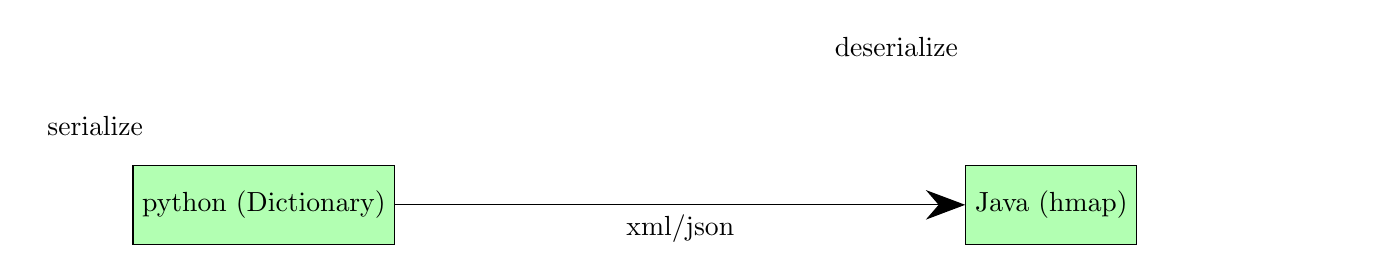
\begin{tikzpicture}[node distance=4cm]
\node (py) [decision] {python (Dictionary)};
\node (java) [decision, below of=py, xshift=10cm, yshift=4cm] {Java  (hmap)};
\node (ser) [detail, below of=py, xshift=0.5cm, yshift=5cm] {serialize};
\node (dese) [detail, below of=ser, xshift=10cm, yshift=5cm] {deserialize};
\draw [-{Stealth[length=5mm]}] (py) -- node[anchor=north] {xml/json} (java);
\end{tikzpicture}
}
\end{figure}

\section{XML: extensible Markup }
XML elements or nodes:
\begin{tcolorbox}
\begin{python}
<people>
	<person>
		<name>Chuck</name>
		<phone>303 4456</phone>
	</person>
	<person>
		<name>Noah</name>
		<phone>303 4456</phone>
	</person>
</people>
\end{python}
\end{tcolorbox}

\begin{itemize}
\item start tag: $<$name$>$
\item single element : $<$name$>$Chuck$<$/name$>$
\item Complex element: $<$person$>$.....$<$/person$>$
\item attribute: $<$phone \textbf{type="intl"}$>$1 734 303 4456 $<$/phone$>$
\item self closing tag: $<$email hide ="yes"/$>$
\item end tag: $<$name$>$
\end{itemize}

\subsection{XML as a Tree}
\begin{figure}[H]
  \centering
        \resizebox {2.4in} {!} {
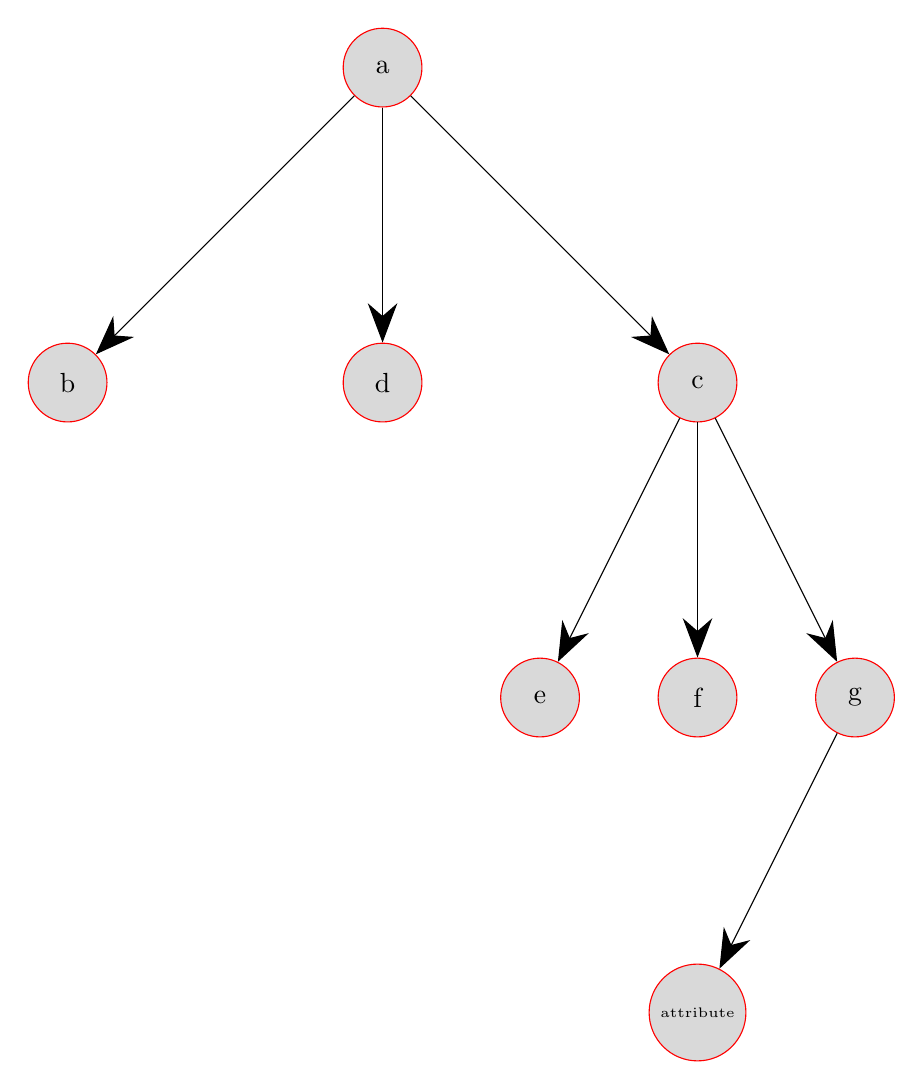
\begin{tikzpicture}[node distance=4cm]
\node (a) [neuron] {a};
\node (b) [neuron, below of=a, xshift=-4cm, yshift=0cm] {b};
\node (c) [neuron, below of=a, xshift=4cm, yshift=0cm] {c};
\node (d) [neuron, below of=a, xshift=0cm, yshift=0cm] {d};
\node (e) [neuron, below of=c, xshift=-2cm, yshift=0cm] {e};
\node (f) [neuron, below of=c, xshift=0cm, yshift=0cm] {f};
\node (g) [neuron, below of=c, xshift=2cm, yshift=0cm] {g};
\node (att) [neuron, below of=f, xshift=0cm, yshift=0cm] {{\tiny attribute}};
\draw[-{Stealth[length=5mm]}] (a) -- (b);
\draw[-{Stealth[length=5mm]}] (a) -- (d);
\draw[-{Stealth[length=5mm]}] (a) -- (c);
\draw[-{Stealth[length=5mm]}] (c) -- (e);
\draw[-{Stealth[length=5mm]}] (c) -- (f);
\draw[-{Stealth[length=5mm]}] (c) -- (g);
\draw[-{Stealth[length=5mm]}] (g) -- (att);
\end{tikzpicture}
}
\end{figure}

\subsection{Parsing XML}
\begin{tcolorbox}
\begin{python}
import xml.etree.ElementTree as ET
data ='''
	<people>
		<name>Chuck</name>
		<phone type="intl"> 1 734 303 4456</phone>
		<email hide="yes"/>
	</person> '''

tree = ET.fromstring(data)
print 'Name:', tree.find('name').text %Chuck
print 'Attr:', tree.find('email').get('hide') %yes
\end{python}
\end{tcolorbox}

\begin{tcolorbox}
\begin{python}
import xml.etree.ElementTree as ET
data ='''
<stuff>
	<users>
		<user x="2">
			<id> 001 </id>
			<name>Chuck</name>
		</user>
		<user x="7">
			<id> 009 </id>
			<name> Brent </name>
		</user>
	<users>
</stuff> '''

stuff = ET.fromstring(data)
lst = stuff.findall( 'users/user' )
print 'User count:', len(lst)
for item in lst
	print 'Name', item.find('name').text
	print 'Id', item.find('id').text
	print 'Attribute', item.get('x').text
\end{python}
\end{tcolorbox}

\section{JSON}
Syntax: JSON represents data as nested lists and dictionaries.
\subsection{Example I}
\begin{tcolorbox}
\begin{python}
import json

data =''' {  %data is a disctionary here '{'
			"name": "Chuck",  % key=name, value = string
			"phone": { 
				"type": "intl",
				"number": "1+ 734 303 4456",
			},
			"email": {
				"hide": "yes",
			}
		}'''

info = json.loads(data) % deserialize/parsing (info is a disctionary)
print "Name:", info["name"]  % Return Chuck
print "Hide:", info["email"]["hide"]  % Return yes
\end{python}
\end{tcolorbox}

\subsection{Example II}
\begin{tcolorbox}
\begin{python}
import json

input =''' [  %data is an array '['
			{ "id": "001", %this is a dictionary
				"x": "2",
				"name": "Chuck",
			},
			{ "id": "009",
				"x": "7",
				"name": "Chuck",
			},
		]'''

info = json.loads(input) % deserialize/parsing (info is a disctionary)
print "User count:", len(info)
for item in info:
	print 'Name:', item['name']
	print 'Id:', item['id']
	print 'Attribute:', item['x']
\end{python}
\end{tcolorbox}

\part{Accessing APIs in python}
API defined set of rules to interface with an application (Google Geocoding API, Twitter API)
\section{Google GeoCoding API: get long/lat of a location}
We start with a url:\\
http://maps.googleapis.com/maps/api/geocode/json?sensor=false\&address=Ann+Arbor\%2C+MI \\

\begin{tabular}{r|l}
\hline
The actual adress & Ann+Arbor\%2C+MI \\
\hline
+ & =space \\
\hline
2\%C & = comma \\
\hline
\end{tabular}

\begin{tcolorbox}
\begin{python}
import urllib
import json

serviceurl = 'http://maps.googleapis.com/maps/api/geocode/json?'

while true:
	address = raw_input('Enter location: ') %Enter location
	if len(address) < 1: break
	
	url = serviceurl 
	+ urllibe.urlencode({'sensor':'false', 'address':adress}) 
	%encode the user input as compatible with API
	print 'Retrieving', url
	uh = urllib.urlopen(url)
	data = uh.read() %read json
	print 'Retrieved', len(data), 'characters'
	
	try: js = json.loads(str(data)) 
	except: js = None
	if 'status' not in js or js['status'] != ' OK': 
		%reading the status = 'OK'
		print '=== Failure To Retrieve ==='
		print data
		continue
	
	print json.dumps(js, indent=4) %make the js readable with indentation
	
	lat = js["results"][0]["geometry"]["location"]["lat"]
	lng = js["results"][0]["geometry"]["location"]["lng"]
	print 'lat', lat, 'lng',lng
	location = js['results'][0]['formatted address']
	print location
\end{python}
\end{tcolorbox}

\section{Twitter API}
Twitter requires to get access token to use API for an application :

\begin{tcolorbox}
\begin{python}
%hidden.py
def oauth() :
	return {
		"consumer_key" : "h7Lu....Ng",
		"consumer_secret" : "dNKen....7Q",
		"token_key" : "10013322....NPAR",
		"token_secret" : "H0yc....qoIp",
	}
\end{python}
\end{tcolorbox}

\begin{tcolorbox}
\begin{python}
%twurl.py= 
import urllib
import oauth
import hidden
	def augment(url,parameters) :
	secrets = hidden.oauth()
	consumer = oauth.OAuthconsumer(secrets['consumer_key'], 
	secrets['consumer_secret'])
	token = oauth.OauthToken(secrets['token_key'], 
	secrets['token_secret']
	oauth_request = oauth.OAuthrequest.from_consumer_and_token(consumer, 
	token=token, http_method='GET', http_url=url, parameters=parameters)
	oauth_request.sign_request(oauth.OAUthSignatureMethod_HMAC_SHA1(), 
	consumer, token)
	return oauth_request.to_url()
\end{python}
\end{tcolorbox}
Return: http://api.twitter.com/1.1/statuses/user\_timeline.json?count=2\\
\&oauth\_version=1.0\&oauth\_token=.....oauth\_consumer..etc

\begin{tcolorbox}
\begin{python}
%twtest.py= 
import urllib
from twurl import augment

print '* Calling Twitter ...'
url = augment('https://api.twitter/1.1/statuses/user_timeline.json',
 {'screen_name': 'drchuck', 'count': '2'} )
% the first part of the url is our request for 2 user_timelines of dr-chuck 
%the 2nd part is the signature
print url
connection = urllib.urlopen(url)
data = connection.read()
print data
headers = connection.info().dict
print headers
\end{python}
\end{tcolorbox}

\end{document}
